% !TEX root =./main.tex

\section{Block 1: Noise Removal, Bandwidth Limiting, and Bias Correction - Stentiford}

This block carries out three functions: it removes the DC bias inherent to the sensors, reduces the noise
 in the signal, and limits the bandwidth to only that which is needed. This is accompished in three stages:
 preliminary debiasing through the very simple method of subtracting the average value of each sensor channel,
 a high-pass filter to fully remove bias and very low-frequency noise, and a low-pass filter to clamp the
 bandwidth at 20kHz and remove any high-frequency noise. 

\begin{figure}[H]
    \centering
    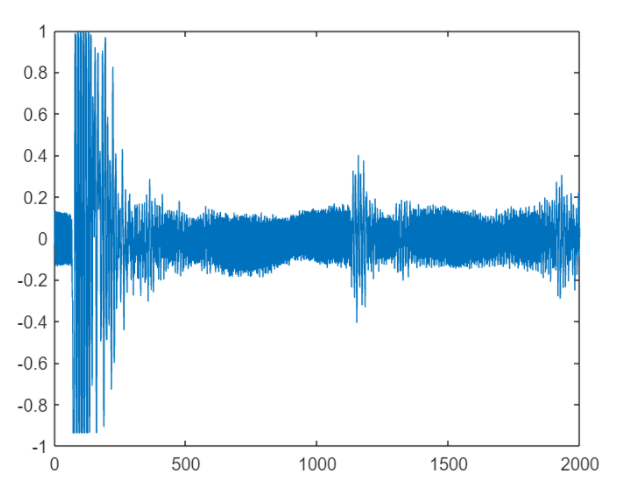
\includegraphics[width=0.5\linewidth]{figures/prefiltered.PNG}
    \caption{Pre-filtered average subtracted only}
\end{figure}
 
The low-pass filter was a 30-order Tukey window filter
with an alpha of 0.5 and a cutoff frequency of 22.16kHz. Its stopband lobes are aligned such that the 25kHz
"jamming" falls directly into one of the cracks. The high-pass filter, meanwhile, is a 61-order least-squares
 filter with a cutoff which targets only the DC component. Using two cascaded filters resulted in a lower total
 order than a single bandpass filter.

\begin{figure}[H]
    \centering
    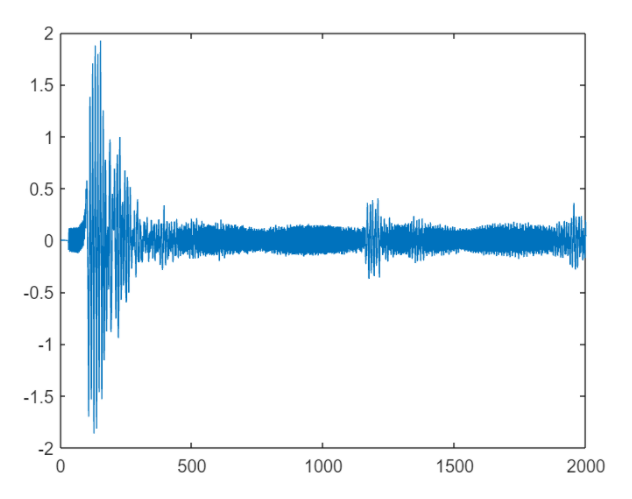
\includegraphics[width=0.5\linewidth]{figures/debiased.PNG}
    \caption{High-pass filtered, DC bias removed}
\end{figure}

An infinite impulse response (IIR) filter, specifically an elliptic filter, would allow for a much lower-order
 filter which would be faster to run, but the need to preserve phase relations meant we restricted ourselves to
 finite impulse response filters to be on the safe side, as FIR filters ensure a linear phase response. Elliptic
 IIR filters do not distort phase too badly, but enough that some amount of distortion is visible in the final
 display.

\begin{figure}[H]
    \centering
    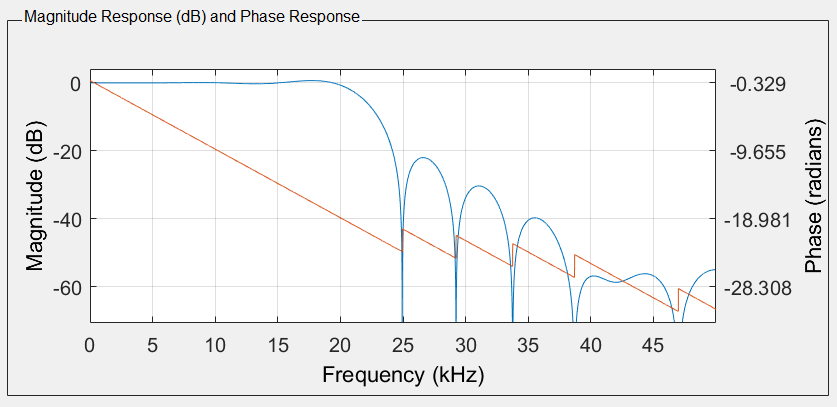
\includegraphics[width=0.5\linewidth]{figures/tukey.PNG}
    \caption{Pre-filtered average subtracted only}
\end{figure}

\begin{figure}[H]
    \centering
    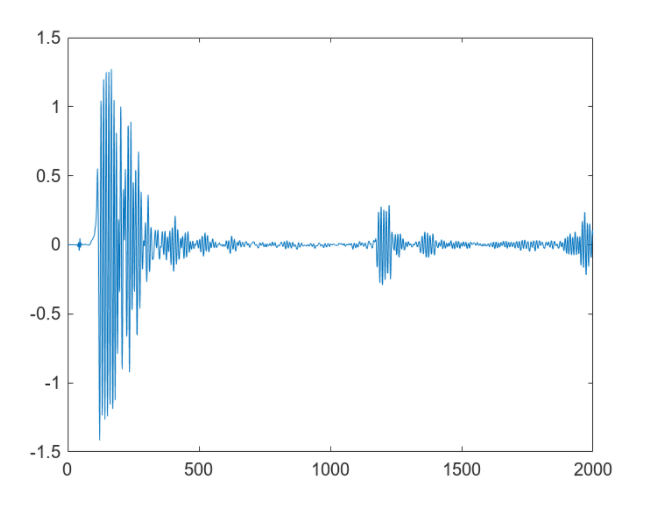
\includegraphics[width=0.5\linewidth]{figures/denoised.PNG}
    \caption{Low-pass filtered, high frequencies removed}
\end{figure}

We decided to place this block first, as the noise-reduced signal is much simpler to deal with when implementing
 the calibration stage than the raw data signal.